\chapter{Probability}

\begin{description}
    \item[Sample space] \marginnote{Sample space}
        Set $\Omega$ of all possible worlds.
        \begin{descriptionlist}
            \item[Event] \marginnote{Event}
                Subset $A \subseteq \Omega$.
            \item[Sample point/Possible world/Atomic event] \marginnote{Sample point}
                Element $\omega \in \Omega$.
        \end{descriptionlist}

    \item[Probability space] \marginnote{Probability space}
        A probability space/model is a function $\prob{\cdot}: \Omega \rightarrow [0, 1]$ assigned to a sample space such that:
        \begin{itemize}
            \item $0 \leq \prob{\omega} \leq 1$
            \item $\sum_{\omega \in \Omega} \prob{\omega} = 1$
            \item $\prob{A} = \sum_{\omega \in A} \prob{\omega}$
        \end{itemize}

    \item[Random variable] \marginnote{Random variable}
        A function from an event to some range (e.g. reals, booleans, \dots).

    \item[Probability distribution] \marginnote{Probability distribution}
        For any random variable $X$:
        \[ \prob{X = x_i} = \sum_{\omega \text{ st } X(\omega)=x_i} \prob{\omega} \]

    \item[Proposition] \marginnote{Proposition}
        Event where a random variable has a certain value.
        \[ a = \{ \omega \,\vert\, A(\omega) = \texttt{true} \} \]
        \[ \lnot  a = \{ \omega \,\vert\, A(\omega) = \texttt{false} \} \]
        \[ (\texttt{Weather} = \texttt{rain}) = \{ \omega \,\vert\, B(\omega) = \texttt{rain} \} \]

    \item[Prior probability] \marginnote{Prior probability}
        Prior/unconditional probability of a proposition based on known evidence.
        
    \item[Probability distribution (all)] \marginnote{Probability distribution (all)}
        Gives all the probabilities of a random variable.
        \[ \textbf{P}(A) = \langle \prob{A=a_1}, \dots, \prob{A=a_n} \rangle \]
    
    \item[Joint probability distribution] \marginnote{Joint probability distribution}
        The joint probability distribution of a set of random variables gives 
        the probability of all the different combinations of their atomic events.

        Note: Every question on a domain can, in theory, be answered using the joint distribution.
        In practice, it is hard to apply.

        \begin{example}
            $\textbf{P}(\texttt{Weather}, \texttt{Cavity}) = $
            \begin{center}
                \small
                \begin{tabular}{|c | c|c|c|c|}
                    \cline{2-5}
                    \multicolumn{1}{c|}{}    & \texttt{Weather=sunny} & \texttt{Weather=rain} & \texttt{Weather=cloudy} & \texttt{Weather=snow} \\
                    \hline
                    \texttt{Cavity=true}    & 0.144 & 0.02 & 0.016 & 0.02 \\
                    \hline
                    \texttt{Cavity=false}   & 0.576 & 0.08 & 0.064 & 0.08 \\
                    \hline
                \end{tabular}
            \end{center}
        \end{example}

    \item[Probability density function] \marginnote{Probability density function}
        The probability density function (PDF) of a random variable $X$ is a function $p: \mathbb{R} \rightarrow \mathbb{R}$
        such that:
        \[ \int_{\mathcal{T}_X} p(x) \,dx = 1 \]
        \begin{descriptionlist}
            \item[Uniform distribution] \marginnote{Uniform distribution}
                \[ 
                    p(x) = \text{Unif}[a, b](x) = 
                    \begin{cases}
                        \frac{1}{b-a} & a \leq x \leq b \\
                        0 & \text{otherwise}
                    \end{cases} 
                \]
            \item[Gaussian (normal) distribution] \marginnote{Gaussian (normal) distribution}
                \[ \mathcal{N}(\mu, \sigma^2) = \frac{1}{\sigma\sqrt{2\pi}}e^{\frac{-(x-\mu)^2}{2\sigma^2}} \]

                $\mathcal{N}(0, 1)$ is the standard Gaussian.
        \end{descriptionlist}

    \item[Conditional probability] \marginnote{Conditional probability}
        Probability of a prior knowledge with new evidence:
        \[ \prob{a \vert b} = \frac{\prob{a \land b}}{\prob{b}} \]
        The product rule gives an alternative formulation:
        \[ \prob{a \land b} = \prob{a \vert b}{\prob{b}} = \prob{b \vert a}{\prob{a}} \]

        \begin{description}
            \item[Chain rule] \marginnote{Chain rule}
                Successive application of the product rule:
                \[ 
                    \begin{split}
                        \textbf{P}(X_1, \dots, X_n) &= \textbf{P}(X_1, \dots, X_{n-1}) \textbf{P}(X_n \vert X_1, \dots, X_{n-1}) \\
                            &= \textbf{P}(X_1, \dots, X_{n-2}) \textbf{P}(X_{n-1} \vert X_1, \dots, X_{n-2}) \textbf{P}(X_n \vert X_1, \dots, X_{n-1}) \\
                            &= \prod_{i=1}^{n} \textbf{P}(X_i \vert X_1, \dots, X_{i-1})
                    \end{split}  
                \]
        \end{description}

    \item[Independence] \marginnote{Independence}
        Two random variables $A$ and $B$ are independent ($A \perp B$) iff:
        \[ 
            \textbf{P}(A \vert B) = \textbf{P}(A) \,\text{ or }\, 
            \textbf{P}(B \vert A) = \textbf{P}(B) \,\text{ or }\,
            \textbf{P}(A, B) = \textbf{P}(A)\textbf{P}(B)
        \]

    \item[Conditional independence] \marginnote{Conditional independence}
        Two random variables $A$ and $B$ are conditionally independent iff:
        \[ \textbf{P}(A \,\vert\, C, B) = \textbf{P}(A \,\vert\, C) \]
\end{description}



\section{Inference with full joint distributions}
Given a joint distribution, the probability of any proposition $\phi$ 
can be computed as the sum of the atomic events where $\phi$ is true:
\[ \prob{\phi} = \sum_{\omega:\, \omega \models \phi} \prob{\omega} \]

\begin{example}
    Given the following joint distribution:
    \begin{center}
        \begin{tabular}{|c|c|c|c|c|}
            \cline{2-5}
            \multicolumn{1}{c|}{}    & \multicolumn{2}{c|}{\texttt{toothache}} & \multicolumn{2}{c|}{$\lnot$\texttt{toothache}} \\
            \cline{2-5}
            \multicolumn{1}{c|}{}    & \texttt{catch} & $\lnot$\texttt{catch} & \texttt{catch} & $\lnot$\texttt{catch} \\
            \hline
            \texttt{cavity}         & 0.108 & 0.012 & 0.072 & 0.008 \\
            \hline
            $\lnot$\texttt{cavity}  & 0.016 & 0.064 & 0.144 & 0.576 \\
            \hline
        \end{tabular}
    \end{center}

    We have that:
    \begin{itemize}
        \item $\prob{\texttt{toothache}} = 0.108 + 0.012 + 0.016 + 0.064 = 0.2$
        \item $\prob{\texttt{cavity} \vee \texttt{toothache}} = 0.108 + 0.012 + 0.072 + 0.008 + 0.016 + 0.064 = 0.28$
        \item $\prob{\lnot\texttt{cavity} \,\vert\, \texttt{toothache}} = \frac{\prob{\lnot\texttt{cavity} \land \texttt{toothache}}}{\prob{\texttt{toothache}}} =
                \frac{0.016 + 0.064}{0.2} = 0.4$
    \end{itemize}
\end{example}

\begin{description}
    \item[Marginalization] \marginnote{Marginalization}
        The probability that a random variable assumes a specific value is given by 
        the sum off all the joint probabilities where that random variable assumes the given value.
        \begin{example}
            Given the joint distribution:
            \begin{center}
                \small
                \begin{tabular}{|c | c|c|c|c|}
                    \cline{2-5}
                    \multicolumn{1}{c|}{}    & \texttt{Weather=sunny} & \texttt{Weather=rain} & \texttt{Weather=cloudy} & \texttt{Weather=snow} \\
                    \hline
                    \texttt{Cavity=true}    & 0.144 & 0.02 & 0.016 & 0.02 \\
                    \hline
                    \texttt{Cavity=false}   & 0.576 & 0.08 & 0.064 & 0.08 \\
                    \hline
                \end{tabular}
            \end{center}
            We have that $\prob{\texttt{Weather}=\texttt{sunny}} = 0.144 + 0.576$
        \end{example}
    \item[Conditioning] \marginnote{Conditioning}
        Adding a condition to a probability (reduction and renormalization).

    \item[Normalization] \marginnote{Normalization}
        Given a conditional probability distribution $\textbf{P}(A \vert B)$,
        it can be formulated as:
        \[ \textbf{P}(A \vert B) = \alpha\textbf{P}(A, B) \]
        where $\alpha$ is a normalization constant.
        In fact, fixed the evidence $B$, the denominator to compute the conditional probability is the same for each probability.

        \begin{example}
            Given the joint distribution:
            \begin{center}
                \begin{tabular}{|c|c|c|c|c|}
                    \cline{2-5}
                    \multicolumn{1}{c|}{}    & \multicolumn{2}{c|}{\texttt{toothache}} & \multicolumn{2}{c|}{$\lnot$\texttt{toothache}} \\
                    \cline{2-5}
                    \multicolumn{1}{c|}{}    & \texttt{catch} & $\lnot$\texttt{catch} & \texttt{catch} & $\lnot$\texttt{catch} \\
                    \hline
                    \texttt{cavity}         & 0.108 & 0.012 & 0.072 & 0.008 \\
                    \hline
                    $\lnot$\texttt{cavity}  & 0.016 & 0.064 & 0.144 & 0.576 \\
                    \hline
                \end{tabular}
            \end{center}

            We have that:
            \[
                \textbf{P}(\texttt{Cavity} \vert \texttt{toothache}) = 
                    \langle 
                        \frac{\prob{\texttt{cavity}, \texttt{toothache}, \texttt{catch}}}{\prob{\texttt{toothache}}},
                        \frac{\prob{\lnot\texttt{cavity}, \texttt{toothache}, \lnot\texttt{catch}}}{\prob{\texttt{toothache}}}
                    \rangle  
            \]
        \end{example}

    \item[Probability query] \marginnote{Probability query}
        Given a set of query variables $\bm{Y}$, the evidence variables $\vec{e}$ and the other hidden variables $\bm{H}$,
        the probability of the query can be computed as:
        \[ 
            \textbf{P}(\bm{Y} \vert \bm{E}=\vec{e}) = \alpha \textbf{P}(\bm{Y}, \bm{E}=\vec{e})
                = \alpha \sum_{\vec{h}} \textbf{P}(\bm{Y}, \bm{E}=\vec{e}, \bm{H}=\vec{h})
        \]
        The problem of this approach is that it has exponential time and space complexity
        that makes it not applicable in practice.

        To reduce the size of the variables, conditional independence can be exploited.
        \begin{example}
            Knowing that $\textbf{P} \models (\texttt{Catch} \perp \texttt{Toothache} \vert \texttt{Cavity})$,
            we can compute the distribution $\textbf{P}(\texttt{Toothache}, \texttt{Catch}, \texttt{Cavity})$ as follows:
            \[
                \begin{split}
                    \textbf{P}&(\texttt{Toothache}, \texttt{Catch}, \texttt{Cavity}) = \\
                        &= \textbf{P}(\texttt{Toothache} \,\vert\, \texttt{Catch}, \texttt{Cavity})
                            \textbf{P}(\texttt{Catch} \,\vert\, \texttt{Cavity}) \textbf{P}(\texttt{Cavity}) \\
                        &= \textbf{P}(\texttt{Toothache} \,\vert\, \texttt{Cavity})
                            \textbf{P}(\texttt{Catch} \,\vert\, \texttt{Cavity}) \textbf{P}(\texttt{Cavity})
                \end{split}
            \]
            $\textbf{P}(\texttt{Toothache}, \texttt{Catch}, \texttt{Cavity})$ has 7 independent values that grows exponentially
            ($2 \cdot 2 \cdot 2 = 8$ values, but one of them can be omitted as a probability always sums up to 1).

            $\textbf{P}(\texttt{Toothache} \,\vert\, \texttt{Cavity}) \textbf{P}(\texttt{Catch} \,\vert\, \texttt{Cavity}) \textbf{P}(\texttt{Cavity})$
            has 5 independent values that grows linearly ($4 + 4 + 2 = 10$, but a value of $\textbf{P}(\texttt{Cavity})$ can be omitted.
            The conditional probabilities require two tables (one for each prior) each with 2 values, 
            but for each table a value can be omitted, therefore requiring $2$ independent values per conditional probability instead of $4$).
        \end{example}
\end{description}



\section{Bayesian networks}

\begin{description}
    \item[Bayes' rule] \marginnote{Bayes' rule}
        \[ \prob{a \,\vert\, b} = \frac{\prob{b \,\vert\, a} \prob{a}}{\prob{b}} \]

    \item[Bayes' rule and conditional independence]
        Given the random variables $\texttt{Cause}$ and\\
        $\texttt{Effect}_1, \dots, \texttt{Effect}_n$, with $\texttt{Effect}_i$ independent from each other,
        we can compute $\textbf{P}(\texttt{Cause}, \texttt{Effect}_1, \dots, \texttt{Effect}_n)$ as follows:
        \[ 
            \textbf{P}(\texttt{Cause}, \texttt{Effect}_1, \dots, \texttt{Effect}_n) = 
            \left(\prod_i \textbf{P}(\texttt{Effect}_i \,\vert\, \texttt{Cause})\right) \textbf{P}(\texttt{Cause})
        \]
        The number of parameters is linear.

        \begin{example}
            Knowing that $\textbf{P} \models (\texttt{Catch} \perp \texttt{Toothache} \vert \texttt{Cavity})$:
            \[
                \begin{split}
                    \textbf{P}&(\texttt{Cavity} \,\vert\, \texttt{toothache} \land \texttt{catch}) \\
                        &= \alpha\textbf{P}(\texttt{toothache} \land \texttt{catch} \,\vert\, \texttt{Cavity})\textbf{P}(\texttt{Cavity}) \\
                        &= \alpha\textbf{P}(\texttt{toothache} \,\vert\, \texttt{Cavity})
                            \textbf{P}(\texttt{catch} \,\vert\, \texttt{Cavity})\textbf{P}(\texttt{Cavity}) \\
                \end{split}
            \]
        \end{example}

    \item[Bayesian network] \marginnote{Bayesian network}
        Graph for conditional independence assertions and a compact specification of full joint distributions.
        \begin{itemize}
            \item Directed acyclic graph.
            \item Nodes represent variables.
            \item The conditional distribution of a node is given by its parents 
                \[ \textbf{P}(X_i \,\vert\, \texttt{parents}(X_i)) \]
                In other words, if there is an edge from $A$ to $B$, then $A$ (cause) influences $B$ (effect).
        \end{itemize}

        \begin{description}
            \item[Conditional probability table (CPT)] \marginnote{Conditional probability table (CPT)}
                In the case of boolean variables, the conditional distribution of a node can be represented using 
                a table by considering all the combinations of the parents.

                \begin{example} 
                    Given the boolean variables $A$, $B$ and $C$, with $C$ depending on $A$ and $B$, we have that:\\
                    \begin{minipage}{.48\linewidth}
                        \centering
                        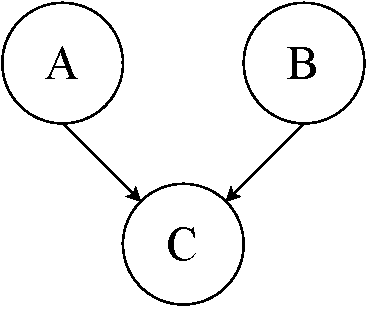
\includegraphics[width=0.35\linewidth]{img/_cpt_graph.pdf}
                    \end{minipage}
                    \begin{minipage}{.48\linewidth}
                        \centering
                        \begin{tabular}{c|c|c|c}
                            A           & B         & $\prob{c \vert A, B}$ & $\prob{\lnot c \vert A, B}$ \\
                            \hline
                            a           & b         & $\alpha$ & $1-\alpha$ \\
                            $\lnot$a    & b         & $\beta$ & $1-\beta$ \\
                            a           & $\lnot$b  & $\gamma$ & $1-\gamma$ \\
                            $\lnot$a    & $\lnot$b  & $\delta$ & $1-\delta$ \\
                        \end{tabular}
                    \end{minipage}
                \end{example}
        \end{description}

    \item[Reasoning patterns] \marginnote{Reasoning patterns}
        Given a Bayesian network, the following reasoning patterns can be used:
        \begin{descriptionlist}
            \item[Causal] \marginnote{Causal reasoning}
                To make a prediction. From the cause, derive the effect.
                \begin{example}
                    Knowing $\texttt{Intelligence}$, it is possible to make a prediction of $\texttt{Letter}$.
                    \begin{center}
                        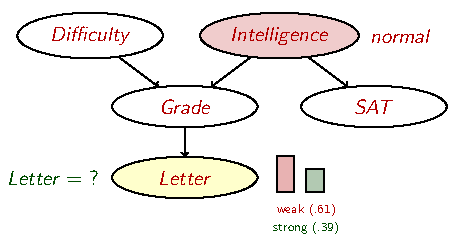
\includegraphics[width=0.5\linewidth]{img/_causal_example.pdf}
                    \end{center}
                \end{example}

            \item[Evidential] \marginnote{Evidential reasoning}
                To find an explanation. From the effect, derive the cause.
                \begin{example}
                    Knowing $\texttt{Grade}$, it is possible to explain it by estimating\\$\texttt{Intelligence}$.
                    \begin{center}
                        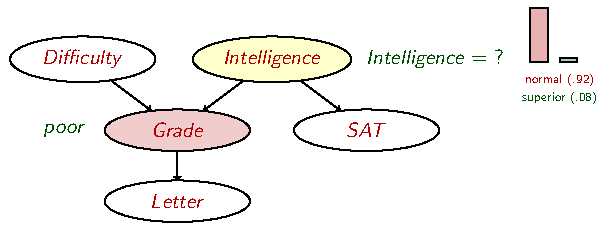
\includegraphics[width=0.65\linewidth]{img/_evidential_example.pdf}
                    \end{center}
                \end{example}

            \item[Explain away] \marginnote{Explain away reasoning}
                Observation obtained "passing through" other observations.
                \begin{example}
                    Knowing $\texttt{Difficulty}$ and $\texttt{Grade}$, 
                    it is possible to estimate \\$\texttt{Intelligence}$.

                    Note that if $\texttt{Grade}$ was not known, 
                    $\texttt{Difficulty}$ and $\texttt{Intelligence}$ would be independent.
                    \begin{center}
                        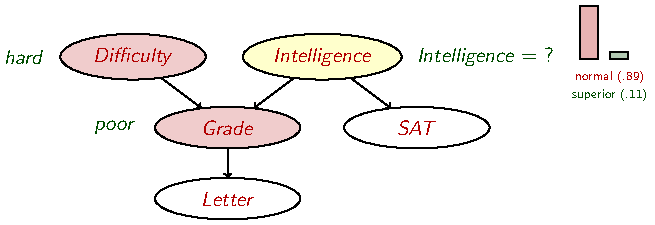
\includegraphics[width=0.70\linewidth]{img/_explainaway_example.pdf}
                    \end{center}
                \end{example}
        \end{descriptionlist}

    \item[Global semantics] \marginnote{Global semantics}
        Given a Bayesian network, the full joint distribution can be defined as
        the product of the local conditional distributions:
        \[ \prob{x_1, \dots, x_n} = \prod_{i=1}^{n} \prob{x_i \,\vert\, \texttt{parents}(X_i)} \]

        \begin{example}
            Given the following Bayesian network:

            \begin{minipage}{.3\linewidth}
                \centering
                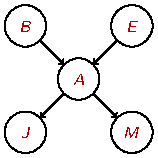
\includegraphics[width=0.7\linewidth]{img/_global_semantics_example.pdf}
            \end{minipage}
            \begin{minipage}{.6\linewidth}
                \[ 
                    \begin{split}
                        &\prob{j \land m \land a \land \lnot b \land \lnot e} \\
                            &= \prob{\lnot b} \prob{\lnot e} \prob{a \,\vert\, \lnot b, \lnot e}
                                \prob{j \,\vert\, a} \prob{m \,\vert\, a}
                    \end{split}
                \]
            \end{minipage}
        \end{example}

    \item[Independence] \marginnote{Bayesian network independence}
        Intuitively, an effect is independent from a cause, 
        if there is another cause in the middle whose value is already known.
        \begin{example}
            \phantom{}

            \begin{minipage}{.3\linewidth}
                \centering
                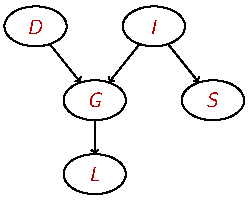
\includegraphics[width=0.75\linewidth]{img/_independence_example.pdf}
            \end{minipage}
            \begin{minipage}{.6\linewidth}
                \[ \textbf{P} \models (\texttt{L} \perp \texttt{D}, \texttt{I}, \texttt{S} \,\vert\, \texttt{G}) \]
                \[ \textbf{P} \models (\texttt{S} \perp \texttt{L} \,\vert\, \texttt{G}) \]
                \[ \textbf{P} \models (\texttt{S} \perp \texttt{D}) \text{ but } 
                    \textbf{P} \models (\texttt{S} \,\cancel{\perp}\, \texttt{D} \,\vert\, \texttt{G}) \text{ (explain away)} \]
            \end{minipage}
        \end{example}
\end{description}